\subsection{Storia della Blockchain}
La prima blockchain fu introdotta, nel 2008, ad opera di Satoshi Nakamoto (pseudonimo di un autore la cui identità è tuttora sconosciuta), e implementata l'anno seguente, con l'obiettivo di fungere da "libro mastro" (registro di tutte le transazioni) della nascente valuta digitale Bitcoin \cite{nakamoto2008bitcoin}. Nel 2009 la creazione di Satoshi Nakamoto, Bitcoin, fu utilizzata per la prima volta per l'acquisto di una pizza. Negli anni successivi, sono nate poi nuove blockchain che hanno preso spunto da questa \cite{blockchain}. Nel 2017, nasce anche Algorand, progetto basato sulla tecnologia blockchain per garantire transazioni scalabili, sicure e decentralizzate attraverso un meccanismo di consenso più rapido, efficiente e meno costoso rispetto a quelli già esistenti.

\subsection{Meccanismi di consenso}
I meccanismi di consenso sono dei procedimenti che avvengono all’interno di una rete distribuita e servono per mettere d’accordo i vari nodi sull’applicazione delle regole e definiscono il protocollo della rete. In questo caso vengono utilizzati per validare le transazioni che sono state effettuate, ma possono servire anche per poter penalizzare chi decide di commettere irregolarità o chi non rispetta queste regole \cite{8632190}.

\subsection{PoW vs PoS}
Il Proof of Work (PoW) e Proof of Stake (PoS) sono due tra gli algoritmi di consenso più famosi nel settore. Il primo è utilizzato da Bitcoin, mentre Proof of Stake è stato adottato da altre criptovalute come Algorand in una versione più efficiente.

\subsubsection{Proof of Work}
Il PoW (Proof of Work) si basa sulla risoluzione di problemi matematici particolarmente complessi da parte della rete, da cui il termine, letteralmente, “prova di lavoro”. Questo meccanismo di consenso sfrutta ciò che in gergo viene definito come “mining”: dei calcolatori molto potenti (detti anche miners) cercano di risolvere un problema matematico complesso al fine di poterne trovare una soluzione chiamata "nonce" e ricevere una ricompensa (ad esempio, un Bitcoin) per il lavoro svolto. Maggiore sarà la potenza di calcolo impiegata, maggiori saranno le possibilità di risolvere il problema matematico in quanto sarà maggiore il numero di tentativi al secondo effettuati. Il problema matematico proposto, infatti, può essere risolto solo per tentativi e il primo miner che trova la soluzione si aggiudica la ricompensa. Tuttavia, l’algoritmo di consenso PoW consente ai miners di convalidare un nuovo blocco e aggiungerlo alla blockchain solo se gli altri nodi della rete concordano con la soluzione fornita dal miner, ripetendo l’operazione risolta.

\subsubsection{Proof of Stake}
Il rapido sviluppo della tecnologia blockchain e delle loro numerose applicazioni emergenti ha ricevuto grande attenzione negli ultimi anni. Il meccanismo del consenso distribuito è la spina dorsale di una rete blockchain e svolge un ruolo chiave nel garantire la sicurezza, l'integrità e le prestazioni della rete. La maggior parte delle attuali reti blockchain ha implementato i meccanismi di consenso Proof of Work, in cui il consenso viene raggiunto attraverso processi di mining intensivi. Tuttavia, questo meccanismo presenta diverse limitazioni, ad esempio inefficienza energetica e scarsa scalabilità. Per superare questi problemi, è stato recentemente sviluppato un nuovo meccanismo di consenso, ovvero il Proof of Stake, che consente di ottenere il consenso dimostrando la proprietà della partecipazione. Questo meccanismo dovrebbe diventare una tecnologia all'avanguardia per le future reti blockchain \cite{nguyen2019proof}. Nel PoS il procedimento fisico attraverso il quale i supercomputer competono tra loro per risolvere problemi matematici complessi, cioè il mining, viene sostituito da un sistema in cui i cosiddetti "validators" garantiscono la validità delle operazioni effettuate impegnando una quota delle proprie criptovalute (dette “stake”). L’idea di base risiede nella necessità di evitare ingenti sprechi di energia e la competizione tra i nodi in merito alle capacità di calcolo. Il principale pregio dei sistemi di PoW risiede proprio nella necessità di impiegare innumerevoli risorse di elettricità ed energia per poter aumentare la potenza di calcolo e risolvere sempre più velocemente i problemi matematici proposti. Questo è ciò che rende il PoW un sistema ad alta affidabilità, in quanto i costi elevati associati al processo di mining rendono, se non impossibile, quantomeno improbabile che i miners investano le proprie risorse per ostacolare il network. Tuttavia, questa caratteristica costituisce anche il principale difetto del PoW \cite{pos}.

\section{Algorand: una Blockchain italiana}
Algorand è una blockchain pubblica completamente permissionless e decentralizzata fondata dal matematico, crittografo e informatico italiano Silvio Micali. Le blockchain permissionless sono quelle in cui chiunque può partecipare al processo di validazione delle transazioni e diventare un nodo della rete. Gli utenti non necessitano l'approvazione di alcuna autorità per unirsi alla rete e chiunque può utilizzare la blockchain per effettuare transazioni e partecipare alla generazione dei blocchi. I dati sono pubblici, quindi tutti i partecipanti possono leggere ogni singolo blocco e hanno facoltà di scrivere una transazione in un blocco futuro. Bitcoin è stata la prima blockchain permissionless che ha ispirato molti a ridefinire l'algoritmo di consenso in un ambiente decentralizzato. In ogni caso, la natura del protocollo Proof of Work ha fatto sì che la capacità di generare i blocchi si sia negli anni progressivamente concentrata tra un numero ristretto di miners. Questo ha portato alla separazione degli utenti in due distinte classi: gli utenti ordinari che utilizzano Bitcoin e i miner professionisti che traggono profitto dalla generazione di nuovi blocchi, questo a causa del fatto che per molti utenti il costo per partecipare alla generazione dei blocchi è divenuto troppo alto \cite{algorand2}.

\subsection{Pure Proof of Stake}
Algorand garantisce che gli utenti non abbiano mai visioni divergenti delle transazioni confermate, anche in presenza di attacchi e se la rete è temporaneamente partizionata. Al contrario, le criptovalute esistenti consentono fork temporanei e quindi richiedono molto tempo, nell'ordine di un'ora, per confermare le transazioni con elevata confidenza. Algorand utilizza un nuovo protocollo di accordo bizantino (BA)\footnote{Il problema dei generali bizantini, in inglese Byzantine Agreement (acronimo di BA) è un problema informatico che consiste nel trovare un accordo, comunicando solo tramite messaggi, tra componenti diversi nel caso in cui siano presenti informazioni discordanti.} per raggiungere il consenso tra gli utenti sulla prossima serie di transazioni. Per scalare il consenso a molti utenti, Algorand utilizza un nuovo meccanismo basato su funzioni casuali verificabili. In questo modo gli utenti sono in grado di verificare privatamente se sono stati selezionati per partecipare alla BA per concordare la prossima serie di transazioni e per includere una prova della loro selezione nei loro messaggi di rete. Nel protocollo BA di Algorand, gli utenti non mantengono alcuno stato privato, il che consente ad Algorand di sostituire i partecipanti immediatamente dopo aver inviato un messaggio. Ciò attenua gli attacchi mirati ai partecipanti scelti dopo che la loro identità è stata rivelata. Valutando le prestazioni di Algorand su 1.000 macchine virtuali EC2\footnote{Amazon Elastic Computer Cloud abbreviato in Amazon EC2, è una parte centrale della piattaforma di cloud computing Amazon Web Services (AWS) di Amazon, che permette agli utenti di affittare macchine virtuali sulle quali eseguire le proprie applicazioni} e simulando fino a 500.000 utenti, i risultati sperimentali mostrano che questa blockchain è in grado di confermare le transazioni in meno di un minuto, raggiungere 125 volte il throughput\footnote{Il throughput è il numero vero di transazioni al secondo che la blockchain è in grado di gestire.} di Bitcoin e non subire quasi nessuna penalità per il ridimensionamento a più utenti.

\subsubsection{Consenso da parte del comitato}
BA ottiene la scalabilità scegliendo un comitato, un piccolo gruppo di rappresentanti selezionati casualmente dall'insieme totale di utenti, per eseguire ogni fase del proprio protocollo. Tutti gli altri utenti osservano i messaggi di protocollo, che consentono loro di apprendere il blocco concordato. BA sceglie i membri del comitato in modo casuale tra tutti gli utenti in base al peso di quest'ultimi. Ciò consente ad Algorand di garantire che una parte sufficiente dei membri del comitato sia onesta. Tuttavia, fare affidamento su un comitato crea la possibilità di attacchi mirati contro i membri del comitato prescelto. Per evitare che un avversario prenda di mira i membri del comitato, BA seleziona i membri in modo privato e non interattivo. Ciò significa che ogni utente nel sistema può determinare in modo indipendente se è stato scelto per far parte del comitato, calcolando una funzione (VRF \cite{814584}) sfruttando la propria chiave privata e delle informazioni pubbliche dalla blockchain. Se la funzione indica che l'utente è stato scelto, restituisce una breve stringa che dimostra l'appartenenza al comitato di questo utente ad altri utenti, che l'utente può includere nei suoi messaggi di rete. Poiché la selezione dell'appartenenza non è interattiva, un avversario non sa quale utente scegliere come target finché quell'utente non inizia a partecipare a BA. Infine, un avversario può prendere come bersaglio un membro del comitato una volta che quel membro ha inviato un messaggio in BA. BA mitiga questo attacco richiedendo ai membri del comitato di parlare solo una volta. Pertanto, una volta che un membro del comitato invia il suo messaggio (esponendo la sua identità a un avversario), il membro del comitato diventa irrilevante per BA. BA raggiunge questa proprietà evitando qualsiasi stato privato (eccetto la chiave privata dell'utente), che rende tutti gli utenti ugualmente in grado di partecipare, ed eleggendo un nuovo comitato per ogni fase del protocollo di accordo bizantino \cite{algorand-bizantine}.

\section{Gli smart contract}
In questa sezione, vedremo cosa sono e come si possono implementare gli smart contract. In generale, sono programmi che vengono archiviati sulla blockchain ed eseguiti quando vengono soddisfatte determinate condizioni; possono generare transazioni di pagamenti e asset, possono anche memorizzare valori sulla blockchain. Quando lo smart contract viene creato, la rete restituirà un application-id (ID) univoco, il quale può quindi essere utilizzato per effettuare chiamate (Application Call) a quest'ultimo. Lo smart contract avrà anche un indirizzo Algorand univoco che viene generato da questo ID che gli permette di fungere da garante tra due o più soggetti per lo scambio di beni quando una certa condizione è stata soddisfatta. In Algorand, gli smart contract possono essere scritti in TEAL o PyTeal; il primo (TEAL) è un linguaggio Turing-completo\footnote{Un linguaggio di programmazione è Turing-complete se la sua semantica permette di implementare una qualsiasi macchina di Turing.} simile ad assembler, il secondo (PyTeal) è una libreria Python per la generazione di programmi TEAL che fornisce una sintassi comoda e familiare.

\subsection{Variabili locali e globali}
Nella fase di creazione di uno smart contract è necessario specificare le variabili utilizzate, che possono essere di due tipologie: stringhe di byte o interi senza segno. Le variabili devono essere specificate sia a livello globale che locale e sono dichiarate come nell'esempio di seguito:

\begin{pythoncode}
#dichiarazione dello stato di memoria dell'applicazione (immutabile)
local_ints = 1
local_bytes = 1
global_ints = 0
global_bytes = 1
global_schema = transaction.StateSchema(global_ints, global_bytes)
local_schema = transaction.StateSchema(local_ints, local_bytes)
\end{pythoncode}

Il numero di variabili che possono essere memorizzate è limitato in base a come è stato creato il contratto la prima volta. Nell'esempio sopra viene creato uno smart contract con due variabili: una locale di tipo intero senza segno e una globale di tipo stringa. Lo spazio della chiave\footnote{La chiave è intesa come il nome della variabile.} è limitato a 64 byte mentre la chiave più il valore può arrivare al massimo a 128 byte totali. L’archiviazione globale è formata dai dati che vengono specificatamente memorizzati sulla blockchain a livello globale. I valori di archiviazione locale vengono archiviati nell'account che ha aderito allo smart contract con la fase di opt-in\footnote{La fase di opt-in avvia la partecipazione di un utente allo smart contract.}.

\subsection{Tipi di smart contract}
Gli smart contract si dividono in due grandi categorie: smart contract detti anche stateful contract e smart signature chiamati anche stateless contract.

\subsubsection{Smart Contract (stateful contract)}
 Gli smart contract sono contratti che, una volta implementati, sono richiamabili in remoto. Una volta distribuita, l'istanza on-chain del contratto prende il nome di "applicazione" a cui viene assegnato un ID univoco. Gli smart contract possono accedere ai valori della blockchain, come i saldi dei conti e i parametri di configurazione delle risorse. Sono in grado anche di eseguire transazioni come parte dell'esecuzione della logica. Ogni applicazione ha un account associato che può contenere Algo (criptovaluta di Algorand)\footnote{L'Algo è la moneta  della rete principale di Algorand, la MainNet.} o ASA (Algorand Standard Asset \cite{asa}). Nel tipo di contratto stateful una certa quantità di spazio di archiviazione sulla blockchain viene utilizzata per memorizzare valori (globalmente o localmente). L'archiviazione dei valori locali si riferisce alla memorizzazione dei valori nel saldo del conto dell'account se l'account ha aderito allo smart contract. Lo storage globale invece è un dato che viene specificamente archiviato sulla blockchain per lo smart contract, a livello globale. In Algorand, uno smart contract è composto da due programmi:
 \begin{itemize}
 \item Approval-Program: è responsabile di tutte le chiamate ad eccezione del Clear-Program.
 \item Clear-Program: questo tipo di programma viene utilizzato per rimuovere lo smart contract dall'account Algorand che lo chiama.
 \end{itemize}
 Entrambi i programmi possono avere successo o fallire, a seconda della logica con cui sono stati implementati. Se una variabile globale o locale viene modificata e il programma ha esito negativo, le modifiche di stato non verranno applicate.
 
\subsubsection{Smart Signature (stateless contract)}
Gli smart signature sono piccoli programmi che vengono inviati come parte di una transazione e valutati al momento dell'invio che contengono la logica utilizzata per firmare le transazioni. Sebbene la logica nello smart signature sia archiviata nella blockchain come parte della risoluzione della transazione, la logica non è richiamabile da remoto. Quando la logica viene inviata a un nodo, l'AVM (Algorand virtual machine)\footnote{L'Algorand virtual machine (AVM) gira su ogni nodo della blockchain di Algorand e si tratta di una macchina virtuale che valuta gli smart contract e gli smart signature rispetto alle transazioni con cui vengono chiamati.} valuta se la condizione codificata dalla logica della smart signature è verificata o meno; nel caso non sia verificata, la transazione associata non verrà eseguita. Una transazione firmata con uno smart signature viene valutata da un nodo Algorand utilizzando la macchina virtuale Algorand (AVM). L'obiettivo principale di questi contratti è quello di approvare (Approve) o rifiutare (Reject) le transazioni.

\subsubsection{Metodi dell'Applicazione}
Le chiamate agli smart contract avvengono utilizzando le transazioni. Di seguito, vediamo tutti i tipi di chiamate:
\begin{enumerate}
    \item Create: metodo che distribuirà l'app. La creazione dell'applicazione restituisce un application-id.
    \item Opt-In: uno user-account (utente Algorand) utilizza questa transazione per iniziare a partecipare ad uno smart contract. La partecipazione attiva l'utilizzo della memoria locale (local storage) dell'utente. Ovviamente per partecipare è necessario conoscere l'application-id che viene restituito dopo la creazione dello smart contract.
    \item Call(NoOp): l'utente può ora iniziare ad usare l'applicazione dopo che nel punto 2 ha partecipato allo smart contract. Questo metodo serve per chiamare/eseguire l'Approval-Program\footnote{L'Approval-Program è responsabile dell'elaborazione di tutte le chiamate allo smart contract, ad eccezione della clear-call eseguita con il Clear-Program. Questo programma è responsabile dell'implementazione della maggior parte della logica dello smart contract.}.
    \item Read State: chiunque può leggere lo stato globale di un'applicazione o lo stato locale di un'applicazione di un certo account utilizzando le API\footnote{API è l'abbreviazione di interfaccia di programmazione delle applicazioni (application programming interface), ovvero un insieme di definizioni e protocolli per la creazione e l'integrazione di software applicativi.}.
    \item UpdateApplication: transazione da eseguire per aggiornare i programmi TEAL di uno smart contract (ovvero l'Approval-Program e il Clear-Program). Il creatore può aggiornare l'Approval-Program usando il metodo di update (ovviamente se l'attuale Approval-Program lo consente). Attenzione, in realtà chiunque può aggiornare il programma, per questo motivo se non si desidera che questo accada è necessario aggiungere del codice per gestire questa situazione, come nel seguente esempio:
    
    \begin{pythoncode}
    program = Assert(Global.creator_address()==Txn.sender())
    print(compileTeal(program, Mode.Application)
    \end{pythoncode}
    % \lstinputlisting[label= updateapp1, caption= Esempio, language=python, basicstyle=\small]{listing/sourceCode/updateapp1.py}
    In alternativa possiamo costruire un codice che restituisca sempre 0 quando viene effettuata una chiamata all'applicazione per impedire a chiunque di aggiornare il codice, come in quest'altro esempio:

    \begin{pythoncode}
    is_not_update = Seq( Return(Int(1))
    program = If (
     OnComplete.UpdateApplication == Txn.on_completion(),
     Return(Int(0)),
     is_not_update
    )
    print(compileTeal(program, Mode.Application)
    \end{pythoncode}
    % \lstinputlisting[label= updateapp2, caption= Esempio, language=python, basicstyle=\small]{listing/sourceCode/updateapp2.py}
    
    \item Close out: l'utente può interrompere l'uso dell'applicazione inviando una transazione di chiusura. Ciò rimuoverà lo stato locale per questa applicazione dell'account dell'utente. Gli utenti utilizzano quindi questa transazione per chiudere la loro partecipazione allo smart contract. Questa chiamata può non riuscire in base alla logica TEAL, impedendo all'account di rimuovere lo smart contract dal balance record (record di saldo).
    \item Delete: transazione che elimina l'applicazione. Chiunque può eliminare uno smart contract, se non si vuole ciò bisogna modificare la logica del programma.
    \item Clear State: simile a Close Out ma la transazione eliminerà sempre lo smart contract dal record del saldo del conto (account balance record) indipendentemente che il programma abbia esito positivo o negativo.
\end{enumerate}

\subsection{Buona programmazione degli smart contract}
Quando si lavora con TEAL per sviluppare smart contract, è necessario seguire alcune linee guida. Ad esempio è consigliato verificare sempre che la proprietà RekeyTo di qualsiasi transazione sia impostata su ZeroAddress a meno che lo smart contract non sia specificamente coinvolto in un'operazione di rekeying. Il rekeying consente di modificare la propria chiave privata senza la necessità di modificare il proprio indirizzo pubblico. Nella maggior parte delle blockchain invece, quando è necessario modificare una chiave privata perchè compromessa, è necessario aprire un nuovo account e spostare le risorse dal vecchio account al nuovo. Per informazioni sulle linee guida è sufficiente visitare la pagina ufficiale \cite{guidelines}.

\section{PyTeal}
Com'è stato accennato in precedenza, PyTeal è una libreria Python per la generazione di programmi TEAL che fornisce una sintassi comoda e familiare.

\subsection{Tipi}
Un'espressione PyTeal può far riferimento a uno dei seguenti tipi di dato: 
\begin{itemize}
    \item uint64, interi senza segno a 64 bit
    \item byte slice, stringhe di bytes
\end{itemize}
Sia i valori delle variabili locali che globali per il contratto corrente possono essere modificati dal codice dello smart contract. 
Vediamo alcuni semplici esempi di codice in grado di creare, aggiornare e eliminare valori nello stato locale o globale. 

\begin{pythoncode}
from pyteal import *

#  variabili globali
program = App.globalPut(Bytes("MyKey"), Int(50))
program = App.globalGet(Bytes("MyKey"))
program = App.globalDel(Bytes("MyKey"))

#  variabili locali
program = App.localPut(Int(0), Bytes("MyKey"), Int(50))
program = App.localGet(Int(0), Bytes("MyKey"))
program = App.localDel(Int(0), Bytes("MyKey"))
print (compileTeal(program, Mode.Application))
\end{pythoncode}
% \lstinputlisting[label= variabili, caption= le variabili, language=python, basicstyle=\small]{listing/sourceCode/localglobalVariable.py}

\subsection{Oggetti di tipo Txn}
Di seguito, descriviamo gli oggetti che è possibile utilizzare nel nostro contratto intelligente:

\begin{enumerate}
    \item Txn: è un oggetto (in particolare un'istanza) che contiene la transazione corrente da valutare per vedere se rispetta lo smart contract
    \item GTxn: è invece un oggetto che contiene un gruppo di transazioni in fase di valutazione (è un'istanza di TxnGroup).
    \item InnerTxn: è un'istanza di TxnObject, contiene la transazione interna inviata più di recente.
\end{enumerate}

\subsection{Seq}
Espressioni multiple possono essere presenti in una sequenza.

\begin{pythoncode}
program = Seq (
    App.globalPut(Bytes("count"), App.globalGet(Bytes("count"))+Int(1)),
    Approve()
)
\end{pythoncode}
% \lstinputlisting[label= seq, caption= Esempio dell'uso di Seq, language=python, basicstyle=\small]{listing/sourceCode/seq.py}

Questo programma conta semplicemente le volte in cui è stato eseguito cioè imposta il conteggio della chiave "count" sul valore che detiene attualmente a cui sommo uno e infine approva. Sfrutta il fatto che App.globalGet restituirà 0 se provi a cercare una chiave che non esiste ancora.

\subsection{Condizioni base: if, then, else, elseif}
\begin{pythoncode}
program = Seq (
    if (App.globalGet(Bytes("count"))==Int(100))
    .then (
        #100esimo chiamante di questa app
        App.globalPut(Bytes("100thCaller"), Txn.sender())
    )
    .else (
        App.globalPut(Bytes("not100thCaller"), Txn.sender())
    ),
    App.globalPut(Bytes("count"), App.globalGet(Bytes("count"))+Int(1)),
    Approve(),
)
\end{pythoncode}

Il programma appena mostrato utilizza tre variabili globali: "count" di tipo uint64, "100thCaller" e "not100thCaller", entrambe di tipo byte slice. Una volta chiamato, il programma controlla che il valore associato a "count" sia uguale a 100 e se questa condizione è verificata, scrive su "100thCaller" l'indirizzo pubblico del mittente della transazione, altrimenti quest'ultimo indirizzo viene scritto sulla variabile "not100Caller". Infine, viene incrementato di uno il valore di "count".

\subsection{Subroutines}
In PyTeal le subroutine sono essenzialmente funzioni o pezzi di codice che possono essere inserite in una funzione Python. E' necessario aggiungere  il decoratore di subroutine e dichiarare il tipo restituito. Di seguito, vediamo un esempio:

\begin{pythoncode}
@Subroutine(TealType.uint64)
def isEven(i) :
    return i%Int(2) == Int(0)
App.globalPut(Bytes("value_is_even"), isEven(Int(10)))
\end{pythoncode}
% \lstinputlisting[label= subroutine1, caption= Esempio subroutine, language=python, basicstyle=\small]{listing/sourceCode/subroutine1.py}

\begin{pythoncode}
@Subroutine(TealType.uint64)
def recursiveisEven(i) :
    return (
        if (i == Int(0)
        .Then ( Int(1)
        .ElseIf ( i == Int(1))
        .Then ( Int(0))
        .Else (recursiveisEven( i-Int(2))
\end{pythoncode}
% \lstinputlisting[label= subroutine2, caption= Esempio subroutine risorsiva, language=python, basicstyle=\small]{listing/sourceCode/subroutine2.py}

Quello che accade è che il codice in fase di compilazione viene archiviato. Ogni volta che viene invocato il metodo, si va alla riga della subroutine, si esegue la funzione e infine si ritorna alla riga del codice in cui eravamo precedentemente.

\subsection{Inner Transaction}
A partire da AVM 1.0 le applicazioni possono creare ed eseguire singole transazioni chiamate "inner-transaction". Le transazioni interne consentono alle applicazioni stateful (smart contract) di avere molti degli effetti di una transazione di primo livello ma la principale differenza è che queste non sono firmate.

\section{Sviluppare con Algorand}
In questa sezione, analizzeremo i tool di sviluppo per Algorand, come collegarsi alla blockchain per ricercare informazioni e come poter scrivere su quest'ultima attraverso le transazioni. Prima di iniziare con gli argomenti appena elencati introduciamo quali sono le tipologie di rete pubbliche disponibili e le loro differenze. In Algorand esistono quattro reti pubbliche: MainNet, BetaNet, TestNet e DevNet. La prima (MainNet) è la rete principale di Algorand con asset a valore reale, inclusa la valuta nativa di Algorand: l'Algo. TestNet rispecchia MainNet in termini di versione del suo protocollo (ovvero software) e la valuta si chiama Algos, disponibile tramite un dispenser, presenta il blocco genesi diverso, il che significa che lo stato dei conti e la distribuzione dei fondi sono differenti. BetaNet è la blockchain in cui verranno rilasciate nuove funzionalità a livello di protocollo per i test iniziali. Pertanto, la qualità e le funzionalità potrebbero non essere definitive e gli aggiornamenti del protocollo e i riavvii della rete sono comuni. DevNet è una rete basata su nightly build\footnote{Le nightly build o build notturne vengono solitamente rilasciate quotidianamente e solitamente di notte, a significare il termine di una giornata lavorativa.}. \cite{algorand_network}.

\subsection{Algorand Sandbox}
La Sandbox di Algorand è un modo rapido per creare e configurare un ambiente di sviluppo Algorand con Algod\footnote{Tramite Algod è possibile eseguire transazioni alla blockchain per la creazione di uno smart contract, effettuare chiamate a quest’ultimo, fare aggiornamenti e cancellazioni e molto altro ancora.} e Indexer\footnote{L'Indexer è lo strumento fornito da Algorand per ricercare informazioni nella blockchain.} ed è disponibile sul portale GitHub\footnote{GitHub è un servizio di hosting per progetti software.}. E' uno strumento fornito da Algorand che semplifica per lo sviluppatore il processo di configurazione di un nodo Algorand in un ambiente containerizzato. Con containerizzazione intendiamo il raggruppamento di codice software e di tutti i relativi componenti necessari, come librerie, framework e altre dipendenze, in modo che risultino isolate in un proprio contenitore che chiamiamo "container". Questo metodo consente di eseguire in modo uniforme il software o l'applicazione contenuta nel container in qualsiasi ambiente e infrastruttura, indipendentemente dal sistema operativo eseguito. Il container costituisce una sorta di bolla, un ambiente di elaborazione circostante all'applicazione, che la mantiene indipendente da ciò che la circonda \cite{containerization}. Per iniziare ad utilizzare la Sandbox è necessario prima clonare la repo da terminale, con il comando:
\begin{pythoncode}
git clone https://github.com/algorand/sandbox.git
\end{pythoncode}
Accertarsi poi che Docker-Compose sia installato e che Docker Desktop sia in esecuzione.

\subsubsection{Configurazioni integrate}
Le seguenti configurazioni vengono fornite di default con Sandbox e possono essere utilizzate eseguendo il comando \textit{./sandbox up <config>} dal terminale, assicurandosi di trovarsi all'interno della cartella "sandbox" appena scaricata. \\ \\
L'elenco delle configurazioni (<config>) di rete privata disponibili sono:
\begin{itemize}
    \item release - build di sviluppo stabile di algod e ramo principale di Indexer.
    \item nightly - build di sviluppo stabile di algod e il ramo di sviluppo di Indexer.
    \item beta - build beta di algod e ramo di sviluppo di Indexer.
    \item dev - ramo di sviluppo di algod e Indexer, la costruzione di algod richiede un po' di tempo, quindi questo avvio sarà più lento rispetto alle altre configurazioni di rete privata.
\end{itemize}
Esiste anche una configurazione (<config>) per ciascuna delle reti di lunga durata:
\begin{itemize}
    \item mainnet
    \item testnet
    \item betanet
    \item devnet
\end{itemize}

\subsubsection{Come usare la Sandbox}
Per avviare la Sandbox e inizializzare la rete privata predefinita, viene utilizzato il comando \textit{./sandbox up}.

\subsection{Algod}
Un'applicazione si connette alla blockchain di Algorand tramite un client Algod che richiede un indirizzo IP e un token Algod valido da un nodo Algorand connesso alla rete con cui prevede di interagire. Tramite Algod è possibile eseguire transazioni alla blockchain per la creazione di smart contract, effettuare chiamate a quest'ultimo, fare aggiornamenti e cancellazioni. E' poi possibile creare asset, aggiornarli, eliminarli o effettuare transazioni ad altri account Algorand. In poche parole è lo strumento che utilizziamo per poter interagire con la blockchain. L'operazione di lettura della blockchain invece la si fa tramite l'indicizzatore (Indexer).

\subsubsection{Instanziare Client Algod SDK}
Per utilizzare il client Algod e potersi connettere alla rete della Testnet è necessario aver avviato la Sandbox con il comando \textit{./sandbox up testnet}.
Fatto ciò, vediamo il codice Python per collegarsi effettivamente al client:
\begin{pythoncode}
from algosdk.v2client import algod

algod_address = "http://localhost:4001"
algod_token = 
"aaaaaaaaaaaaaaaaaaaaaaaaaaaaaaaaaaaaaaaaaaaaaaaaaaaaaaaaaaaaaaaa"
algod_client = algod.AlgodClient(algod_token, algod_address)
\end{pythoncode}

\subsubsection{Alternativa alla Sandbox}
Un'alternativa all'Algorand Sandbox per comunicare con la rete MainNet, BetaNet e TestNet è Purestake: un servizio che offre un’interfaccia sicura per permettere l'utilizzo di Algod e dell’Indexer. Nella versione standard gratuita si ha accesso a tutti i tipi di reti (TestNet, BetaNet e MainNet) e possono essere eseguite 500.000 richieste al giorno, 30 query Algod e 10 query Indexer al secondo. Per poter usufruire del servizio è obbligatorio registrarsi in quanto si richiede una chiave privata (nell'esempio chiamata "my-private-key") per far funzionare il client, fornita dopo l'iscrizione. Di seguito si mette a disposizione il codice base per il collegamento ad Algod della TestNet utilizzando il linguaggio di programmazione Python:
\begin{pythoncode}
headers = {
"X-API-Key": "my-private-key",
}
algod_client = algod.AlgodClient("",
"https://testnet-algorand.api.purestake.io/ps2", headers)
\end{pythoncode}

\subsubsection{Direttiva per Docker}
Per utilizzare Algod (istanziato con la Sandbox) all'interno di un container Docker dobbiamo sostituire "localhost" in algod\_address con "host.docker.internal", poiché vogliamo che il container acceda alla porta host \textit{sandbox 4001}. Mostriamo di seguito questo concetto per maggiore chiarezza:

\begin{pythoncode}
from algosdk.v2client import algod

algod_address = "http://host.docker.internal:4001"
algod_token = 
"aaaaaaaaaaaaaaaaaaaaaaaaaaaaaaaaaaaaaaaaaaaaaaaaaaaaaaaaaaaaaaaa"
algod_client = algod.AlgodClient(algod_token, algod_address)
\end{pythoncode}

\subsection{Indexer}
Per ricercare informazioni nella blockchain di Algorand si fa uso di uno strumento chiamato Indexer V2 (versione 2). Lo scopo principale di questo indicizzatore è fornire un'interfaccia API REST di chiamate API per supportare la ricerca in Algorand Blockchain. Le API REST dell'indicizzatore recuperano i dati blockchain da un database PostgreSQL che deve essere popolato utilizzando la stessa istanza dell'indicizzatore o un'istanza separata dell'indicizzatore che deve connettersi al processo Algod di un nodo Algorand in esecuzione per leggere i dati del blocco [vedi figura \ref{fig: indexer}]. Questo nodo deve essere anche un nodo di archiviazione per rendere possibile la ricerca nell'intera blockchain. L'indicizzatore fornisce una serie di chiamate API REST per la ricerca di transazioni, conti, asset e blocchi sulla blockchain. Ognuna di queste chiamate fornisce anche diversi parametri di filtro per supportare il perfezionamento delle ricerche \cite{algorand_indexer}.

\begin{figure}[!h]
\centering
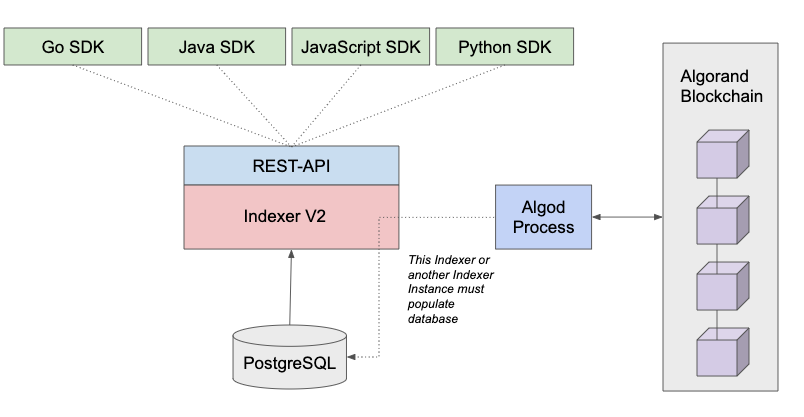
\includegraphics[scale=0.4]{images/indexerv2.png}
\caption{Architettura Indexer V2}
\label{fig: indexer}
\end{figure}

\subsubsection{Instanziare Client Indexer SDK}
La Sandbox non ha lo scopo di fornire un Indexer di TestNet, visto che il suo scopo è di creare un nodo rapido per lo sviluppo di:
\begin{itemize}
    \item una nuova rete privata con un Indexer (che è molto conveniente per la maggior parte dei casi)
    \item un rapido nodo non di archiviazione per TestNet senza Indexer
\end{itemize}

Se si desidera un Indexer TestNet, è necessario eseguire sia un nodo TestNet di archiviazione che un nodo Indexer. Quest'operazione è piuttosto lunga visto che ci vorrà circa una settimana per recuperare tutte le informazioni dalla blockchain e rendere tutto operativo. Per semplificare questo processo è stato utilizzato PureStake: un servizio che offre un'interfaccia sicura all'Indexer V2 di Algorand. Di seguito, si mostra il codice per potersi collegare a questo servizio correttamente:

\begin{pythoncode}
from algosdk.v2client import indexer
headers = {
"X-API-Key": "my-private-key",
}
# instantiate indexer client
myindexer = indexer.IndexerClient("", "https://testnet-algorand.api
.purestake.io/idx2", headers)
\end{pythoncode}

\section{Docker}
Docker è un popolare software libero progettato per eseguire processi informatici in ambienti isolabili, minimali e facilmente distribuibili chiamati container, con l'obiettivo di semplificare i processi di deployment di applicazioni software \cite{docker}. Lo scopo di Docker è quindi quello di rendere più facile la creazione, il deploy e l'esecuzione di applicazioni utilizzando i container. I container consentono allo sviluppatore di pacchettizzare una applicazione con tutte le parti necessarie (le librerie e altre risorse correlate) e consegnarla appunto come un unico pacchetto \cite{docker1}.

\subsection{Le immagini}
Un'immagine Docker è un modello in sola lettura che definisce il container. L'immagine contiene il codice che verrà eseguito, incluse le definizioni per le librerie e le dipendenze necessarie. Un container Docker è un'immagine Docker in esecuzione. Per creare un immagine è necessario creare un particolare file chiamato “Dockerfile”. Il Dockerfile può essere considerato come un manuale di assemblaggio per le immagini. Il suo scopo però non si esaurisce qui. Oltre a specificare come deve essere costruita un’immagine, descrive anche la modalità (di default) con la quale verrà avviato un container a partire da essa. Le istruzioni dichiarate nel Dockerfile verranno eseguite in ordine e, in buona approssimazione, per ognuna di esse verrà generato un layer.

\subsection{Persistenza dei dati}
I container sono pensati per essere distrutti e ricreati più volte a partire dalla stessa immagine. Questo approccio fa parte del concetto di “infrastruttura immutabile” che garantisce lo stesso container ad ogni nuovo deploy. Viene da se che quando si presenta l’esigenza di persistere delle informazioni oltre il ciclo di vita del container o tra più container è necessario avere qualche soluzione che stia al di fuori del container stesso. A dire il vero, è possibile persistere le informazioni anche su un container fino al momento in cui questo container viene distrutto. Tuttavia non è la migliore strategia se poi queste informazioni devono essere disponibili anche al di fuori del contesto di quel singolo container. Per gestire la persistenza dei dati, Docker fornisce due soluzioni:
\begin{itemize}
    \item Volumes: i volumi sono uno spazio creato al di fuori dello Union File System del container che può essere acceduto da più container. Possono essere connessi a più container che ci interagiranno mediante un percorso locale definito da noi.
    \item Bind Mounts: alla stregua dei mount classici di linux, un bind mount è una condivisione di una cartella.
    Con questa tipologia di persistenza, andiamo a condividere una cartella dell’host con il container specificando anche in questo caso a quale path deve accedere in locale per poterci avere accesso \cite{docker_persistenza}.
    \end{itemize}

\subsection{Dockerfile}
Un Dockerfile è un semplice file di testo che, con una sintassi semplice e coincisa, ci permette di esprimere le personalizzazioni che vogliamo apportare ai vari template affinché questi possano diventare delle immagini su misura per noi. 
Di seguito presentiamo le istruzioni più importanti che andranno a comporre questo file.
\begin{description} 
\item[FROM] Tra le tante istruzioni disponibili, FROM è sicuramente quella più importante, nonchè l'unica che non può mai mancare all'interno di ogni Dockerfile. Essa permette di specificare un'immagine di base da cui partire per derivare la nostra immagine personalizzata.
\item[ENV]  Questa istruzione offre la possibilità di impostare variabili di ambiente valide per tutto il contesto di esecuzione di un Dockerfile.
 \item[RUN] Il comando RUN ha lo scopo di eseguire una o più istruzioni definite in formato bash in un nuovo layer. Di fatto aggiungendo un blocco immutabile all’immagine. Se è stato indicato di voler utilizzare Debian come immagine base, possiamo utilizzare l'istruzione RUN per installare un pacchetto tramite il classico comando apt-get.
 \item [CMD] Passiamo ora all’ultima istruzione necessaria per costruire una build, ovvero CMD. CMD è l’istruzione di default per l’esecuzione di un container. Fondamentalmente significa che al run di un container a partire dall’immagine che stiamo definendo, verrà invocata questa istruzione. Ogni Dockerfile ben formato dovrebbe avere al massimo una sola occorrenza di CMD. Ad ogni modo, in presenza di invocazioni multiple, verrà utilizzata solo l’ultima di esse. RUN agisce in fase di build apportando modifiche all’immagine, mentre il comando CMD specifica cosa fare quando viene avviato un container a partire da un’immagine che a tutti gli effetti è già sigillata.
 \item [COPY/ADD] Ci sono poi i comandi COPY e ADD che si occupano di copiare qualcosa dal filesystem dell’host all’interno dell’immagine. Questi due comandi hanno molto in comune. La differenza principale tra i due sta nel fatto che ADD è una sorta di COPY più evoluto, che permette di copiare risorse anche passando un url o decomprimendo direttamente un file qualora venisse riconosciuto come file compresso. 
 \item [EXPOSE] I container, di default non hanno nessuna porta aperta verso l’esterno ed è proprio qui che interviene EXPOSE. Per poter esporre una porta all’esterno, è necessaria la pubblicazione di quella porta relativamente al container che viene istanziato a partire dall’immagine che stiamo descrivendo. Le modalità previste sono due: aperture selettive o aperture generiche. Vediamo solo la prima modalità visto che risulta la più comune. Nell'apertura selettiva, si specifica quindi, quale porta ed eventualmente su quale protocollo viene pubblicata una porta del container verso l’esterno.
 \begin{pythoncode}
 EXPOSE 80/tcp
 EXPOSE 80/udp
 \end{pythoncode}
 Qualora non fosse specificato la porta verrà esposta di default sul protocollo TCP \cite{dockerfile}.
 \item [Altre istruzioni] Sopra sono state mostrate le istruzioni più comuni che sono anche quelle utilizzate all'interno del progetto \cite{dockerbuilder}.
\end{description} 

\subsection{Docker Compose}
Quando si utilizza Docker in modo estensivo, la gestione di diversi contenitori diventa rapidamente difficile da gestire. Docker Compose è uno strumento che ci aiuta a superare questo problema e a gestire facilmente più contenitori contemporaneamente. Con Compose, si utilizza un file YAML per configurare i servizi dell'applicazione. Quindi, con un solo comando, si creano e avviano tutti i servizi. In breve, Docker Compose funziona applicando molte regole dichiarate all'interno di un singolo file di configurazione docker-compose.yml. Quasi ogni regola sostituisce un comando Docker specifico in modo che alla fine dobbiamo solo eseguire:
\begin{pythoncode}
docker-compose up
\end{pythoncode}
Nel file docker-compose.yml è necessario specificare la versione del formato file Compose, almeno un servizio e, facoltativamente, volumi e reti:
\begin{pythoncode}
version: "3.7"
services:
  ...
volumes:
  ...
networks:
  ...
\end{pythoncode}

\subsubsection{Servizi}
I servizi si riferiscono innanzitutto alla configurazione dei container. Ad esempio, consideriamo un'applicazione Web dockerizzata composta da un front-end, un back-end e un database: probabilmente divideremmo quei componenti in tre immagini e li definiremmo come tre diversi servizi nella configurazione:
\begin{pythoncode}
services:
  frontend:
    image: my-vue-app
    ...
  backend:
    image: my-springboot-app
    ...
  db:
    image: postgres
    ...
\end{pythoncode}

\subsubsection{Avvio}
Possiamo avviare il file docker-compose.yml e cioè creare e avviare i container, le reti e i volumi definiti nella configurazione, con il comando seguente:
\begin{pythoncode}
docker-compose up
\end{pythoncode}

\subsubsection{Arresto}
Per interrompere in sicurezza i servizi attivi, possiamo utilizzare il comando \textit{stop}, che conserverà container, volumi e reti, insieme ad ogni modifica apportata agli stessi:
\begin{pythoncode}
docker-compose stop
\end{pythoncode}
Per poterlo riavviare, possiamo semplicemente utilizzare il comando:
\begin{pythoncode}
docker-compose start
\end{pythoncode}
Per resettare lo stato del nostro progetto (distruggerà tutto con la sola eccezione dei volumi esterni), si utilizza il comando:
\begin{pythoncode}
docker-compose down
\end{pythoncode}
\cite{docker-compose}

\subsection{Uso di Docker}
Creando container e avviandoli tramite il docker-compose.yml è possibile farli comunicare senza dover aprire le varie porte. Nel caso si abbia invece la necessità di dover comunicare con un container dall'esterno (ad esempio tramite browser) bisognerà necessariamente aprire manualmente le porte del container.